\usetikzlibrary{positioning}

\centering
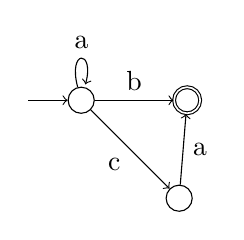
\begin{tikzpicture}
	\coordinate[draw,circle] (q0) at (0,0);
	\coordinate[left=0.5 of q0] (pre);
	\coordinate[draw,double,circle,right=of q0] (qf);
	\coordinate[draw,circle,below right=of q0] (q1);
	\draw[->] (pre) -- (q0);
	\draw[->] (q0) -- node[above] {b} (qf);
	\draw[->] (q0) -- node[below left] {c} (q1);
	\draw[->] (q1) -- node[right] {a} (qf);
	\draw (q0) edge[loop above] node[above] {a} (qf);
\end{tikzpicture}

